\chapter{Analýza problematiky}
V kontexte prezentácií existuje mnoho foriem prezentovania, ako napríklad pracovné pohovory, verejné vystúpenia alebo aj školské prezentácie. Nakoľko zachytiť všetky tieto formy v rámci jedného riešenia je náročné, rozhodol som sa sústrediť sa na iba verejné prezentácie pred publikom.

Pred samotným návrhom riešenia je potrebné pochopiť základné pojmy spojené s prezentáciami a prezentačnými schopnosťami. V nasledujúcich podkapitolách postupne vysvetlím mnou analyzované pojmy úzko spojené s touto problematikou.

\section{Význam prezentácie}
Cieľom prezentácie je často podať informácie poslucháčom alebo publiku za určitým účelom. Tieto účely sú rôzne a každý zdroj uvádza iné množstvo\cite{purposeOfPresentation}. Základné účely sú:
\begin{itemize}
    \item Informovať
    \item Presvedčiť
    \item Inšpirovať
    \item Pobaviť
\end{itemize}
Pre určenie účelu prezentácie je potrebné si uvedomiť, čo chcem prezentáciou dosiahnúť. Príkladom je napríklad, že idem predniesť nový návrh na reklamnú kampaň pre potenciálneho investora. V tomto prípade chcem presvedčiť moje publikum (investorov), že môj nápad je najlepší. Povedzme že chceme znova predniesť nový návrh na reklamnú kampaň predniesť začiatočníkom v oblasti podnikania. Účel tejto prezentácie by bol inšpiratívny.

Podľa tohto účelu prezentácie vie prezentujúci, na aké informácie alebo formu prejavu sa má najviac sústrediť. Napríklad pri informatívnej prezentácii musí prezentujúci využívať prevažne najpodstatnejšie informácie, pri presviedčaní silné fakty, pri inšpirovaní príbehy alebo inak citové prejavy a pre pobavenie vtipné výroky alebo príbehy\cite{purposeOfPresentation}.

\begin{figure}[H]
    \begin{centering}
        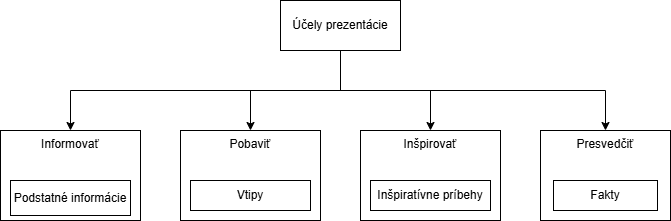
\includegraphics[width=\textwidth]{assets/images/analysis/ucely_prezentacie.png}
        \par\end{centering}
    \caption{Účely prezentácie \label{fig:presentationReasons}}
\end{figure}

\section{Prezentačné schopnosti}
V mojej práci je najpodstatnejšie pochopiť, čo sú to \textbf{prezentačné schopnosti} a čo všetko tento pojem zahŕňa. Prezentačné schopnosti sú vlastnosti a kvality potrebné pre vytváranie a prednášanie presvedčivých prezentácií, ktoré efektívne predávajú informácie a nápady\cite{presentationSkills}. Zahŕňajú nie len hovorené slová ale aj reč tela, vizuálne pomôcky a všeobecnú charizmu prezentujúceho\cite{pressentationSkillsImportance}. Pod vizuálnymi pomôckami si môžeme predstaviť priamo obrazovú prezentáciu, ktorú prezentujúci prednáša.

V mojej práci sa nechcem venovať analýze vizuálnych pomôcok prezentácie, ale sústrediť sa skôr na \textbf{verbálne} a \textbf{neverbálne} aspekty prezentačných schopností, čím docielim zlepšenie samotnej prezentácie. Vizuálne pomôcky sú podstatné pre prezentáciu, no ja sa chcem zamerať na prezentačné schopnosti.

\section{Stavba komunikácie}
Počas mojej analýzy riešenia som narazil na známe pravidlo 7-38-55, ktoré často býva spájané s medziľudskou komunikáciou. Podľa tohto pravidla iba 7 \% významu v komunikácii sprostredkúvajú samotné slová, zatiaľ čo 38 \% pripadá na tón hlasu a až 55 \% na reč tela\cite{73855}. Nakoľko tón hlasu spadá pod neverbálnu komunikáciu, toto pravidlo teda hovorí, že 93\% komunikácie tvorí neverbálna komunikácia.

Hoci je toto pravidlo často citované, v odborných kruhoch býva zároveň aj kritizované. Bolo odvodené z výskumu psychológa Alberta Mehrabiana, ktorý však skúmal veľmi špecifické situácie, predovšetkým rozpory medzi verbálnym a neverbálnym prejavom pri vyjadrovaní emócií. Preto ho nemožno aplikovať univerzálne na všetky formy komunikácie.

Napriek tomu poukazuje na dôležitý fakt, a to že neverbálna zložka komunikácie (napríklad mimika či gestá) má v medziľudskom dorozumievaní výrazný vplyv a neraz môže byť rovnako dôležitá ako samotné slová.

\subsection{Neverbálna komunikácia}
Pod neverbálnou komunikáciou si môžeme predstaviť mnoho vecí. Či už náš postoj, spôsob ako chodíme, výraz tváre, kde máme ruky, no zároveň aj ako rozprávame. V kontexte verejných prezentácií je podstatné nájsť práve také typy neverbálnej komunikácie, ktoré pri nesprávnom vykonávaní nepriaznivo pôsobia na kvalitu prezentácie. Zároveň pri neverbálnej komunikácii je častý problem sebareflexie, pretože tieto prejavy sú často podvedomé, a tým pádom prezentujúci potrebuje dostať spätnú väzbu\cite{intelligentTrainerNguyen}.

Nakoľko negatívne pôsobiacich neverbálnych aspektov je príliž veľa, je potrebné vybrať tie najdôležitejšie. Jeden zo zdrojov vykonal rozhovor s desiatimi expertami v oblasti verejného rozprávania, čo je forma prezentácie, na ktorú som sa rozhodol zamerať\cite{nonverbalImportance}. Po rozhovoroch s odborníkmi zostavili tabľku s údajmi, ktoré rozdelili do viacerých podkategórií.

\begin{figure}[H]
    \begin{centering}
        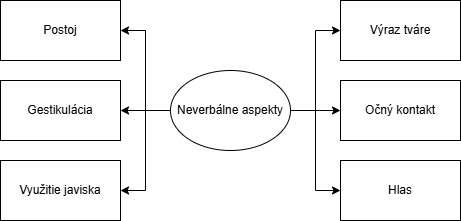
\includegraphics[width=\textwidth]{assets/images/analysis/nonverbals_division.png}
        \par\end{centering}
    \caption{Rozdelenie aspektov neverbálnej komunikácie \label{fig:nonverbalsDivision}}
\end{figure}

Z vyhotovenej tabuľky som vybral tie javy, ktoré najčastejšie spomenuli odborníci a zaradili ich medzi negatívne javy.

\begin{table}[H]
    \centering
    \begin{tabularx}{\textwidth}{|X|X|}
        \hline
        \textbf{Názov javu} & \textbf{Aspekt}  \\
        \hline
        \specialrule{1.2pt}{0pt}{0pt}
        Otočený chrbtom k publiku & Postoj \\ \hline
        Tancovanie (tango a merengue) & Postoj \\ \hline
        Ruky vo vreckach alebo za chrbtom & Postoj \\ \hline
        Žiadna gestikulácia & Gestikulácia \\ \hline
        Držanie / hranie sa s predmetmi & Gestikulácia \\ \hline
        Ruky nad hlavou & Gestikulácia \\ \hline
        "Prázdny" výraz tváre & Výraz tváre \\ \hline
        Žiaden očný kontakt & Očný kontakt \\ \hline
        Státie za počítačom & Využitie javiska \\ \hline
        Konštantný pohyb po javisku & Využitie javiska \\ \hline
        Rozprávanie hlasno pre seba & Hlas \\ \hline
    \end{tabularx}
    \caption{Tabuľka negatívnych javov neverbálnej komunikácie}
    \label{tab:negativeNonverbals}
\end{table}

Jeden z najpodstatnejších aspektov pri verejnom prezentovaní je očný kontakt. Udržiavanie očného kontaktu pomáha pri vytváraní spojenia medzi poslucháčmi, zlepšuje koncentráciu a preukazuje autoritu a sebavedomie\cite{eye_contact}.

Jeden zo zdrojov uvádza, že pri prezentovaní je potrebné využívať signál k zvuku (signal-to-noise). Signál tu definujeme ako akékoľvek pohyby, ktoré dodávajú vášmu rozprávaniu podstatu a ďalej zapájajú publikum, ako napríklad odovzdanie správy rukami alebo očný kontakt s publikom. \cite{nonverbal} Tento pojem znamená, že by prezentujúci mal využívať pohyby spolu s hovoreným slovom. V prípade prepoužívania signálov môže pôsobiť hovorené slovo neprirodzené alebo môžu signály pôsobiť príliš rušivo.

\subsection{Vlastnosti hlasu}
Pri využívani svojho hlasu je potrebné dávať si pozor hneď na niekoľko jeho vlastností. Túto problematiku opisoval v rámci svojej prednášky Julian Treasure\cite{voice} a poukázal na tieto hlasové vlastnosti:
\begin{itemize}
    \item hlasový register
    \item farba hlasu
    \item prozódia
    \item tempo
    \item výška hlasu
    \item hlasitosť
\end{itemize}
Avšak nakoľko detekcia všetkých týchto vlastností hlasu je pomerne komplikovaná, je potrebné z nich vybrať tie najpodstatnejšie. V predošlej sekcii zameranej na neverbálnu komunikáciu odborníci spomenuli niektoré z hore napísaných vlastností hlasu a zároveň aj ako ich negatívne prezentujúci využil. Konkrétne ide o problémy monotónnosti, rýchleho rozprávania a tichého rozprávania.

\subsection{Verbálna komunikácia}
Z hľadiska verbálnej komunikácie sa pri prezentáciach môžeme zamerať na mnoho problémov. S problémami verbalnéj komunikácie je často spôsobená prerušením plynulosti reči, ktorá môže mať viac foriem. Namiesto odprezentovania správne štruktúrovanej reči prezentujúci často hovoria zneistene, opakujú sa a opravújú svoje hovorené slovo.\cite{disfluencies} Častým javom je aj takzvané používanie výplňových slov alebo výplňových zvukov. Niekoľko štúdií preukázalo, že nadmerné používanie výplňových slov alebo zvukov negatívne ovplyvňuje prezentačné zručnosti prezentujúceho.\cite{fillerEffects} \cite{fillerWords} Preto som sa v mojej práci rozhodol venovať sa práve identifikácii týchto slov. V jednom zo zdrojov bolo uvedené, že minimálna prijateľná miera výplňových slov je 1.26 na 100 slov. \cite{fillerWords} Po prekročení tohto limitu začne klesať kredibilita prezentujúceho u poslucháčov.

\section{Časové rady}
Pre pochopenie mojej práce je podstatné pochopiť aj čo sú to časové rady. Časové rady sú jednoducho sekvencie dátových bodov merané v diskrétnych časových bodoch, ktoré sú zoradené chronologicky podľa času\cite{timeSeriesDef}. V mojej práci sa budem zaoberať presne takýmito dátami, nakoľko budem musieť analyzovať jednotlivé vlastnosti hlasu a pohyby používateľa v jednotlivých časových bodoch počas celej prezentácie. Problematika časových radov je pomerne rozsiahlá, no po uvažovaní, ktoré vlastnosti a algoritmy časových radov sa budem sústrediť som sa rozhodol zamerať na dve, a to konkrétne na \textbf{segmentáciu} a \textbf{detekciu trendu}.

\subsection{Segmentácia časových radov}
Segmentácia je rozdeľovanie časových radov na časti, segmenty, ktoré logicky rozdelia dáta\cite{timeSeriesSeg}. Z hľadiska segmentácie je potrebné nájsť také body v časovom rade, ktoré rozdelia dáta podľa odchýlky, priemeru alebo pri zmene trendu. Existuje mnoho algoritmov, ktoré zabezpečujú segmentáciu časových radov. Často sa delia na dve kategórie, a to \textbf{offline} a \textbf{online}. Offline reprezentuje algoritmy, ktoré majú všetky dáta dostupné naraz a online tie, ktoré dáta dostávajú postupne. Ďalšie rozdelenie je podľa spôsobu detekcie bodov zmien, a to sú:
\begin{itemize}
    \item Top-down approach
    \item Bottom-up approach
    \item Sliding window
    \item SWAB (sliding window and bottom-up)
\end{itemize}

Z hľadiska využitia v rámci mojej práce sa môže segmentácia použiť pre rozdelenie dát na úseky, kde ostáva rovnaký trend alebo sa výrazne zmení priemer. Napríklad pri analýze pohybov rúk môže algoritmus rozoznať, že prezentujúci využíva pohyby rúk výrazne v prvej časti prezentácie (trend stúpa alebo je konštantný) a následne ich prestane kvôli tréme využívať (trend klesá). Zároveň body zmien často indikujú anomálie, napríklad prudký pohyb rukami alebo náhle zvýšenie hlasitosti. Tieto údaje môžu byť pre prezentujúceho podstatné, aby si tieto často podvedomé javy uvedomil a zlepšil sa.

\subsection{Detekcia trendu}
Trend je vzor v časovom rade, ktorý sa vyznačuje konzistentným správaním údajov (napríklad stúpajúcim alebo klesajúcim pohybom) v priebehu času\cite{timeSeriesTrend}. V niektorých oblastiach sa trend definuje aj ako všeobecný smer priemeru v dátach\cite{timeSeriesTrendAlgo}.
Pri mojej analýze som narazil na štyri druhy algoritmov na detekciu trendu, ktoré využívajú rozne techniky detekcie, a to:
\begin{itemize}
    \item Fuzzy logic
    \item Štatistické
    \item Regresné
    \item Wavelet
\end{itemize}

Využitie detekcie trendu v rámci mojej práce chcem využiť pri analýze jednotlivých segmentov prezentácie. Napríklad zistím, či v prvom segmente prezentácie prezentujúci prestal postupne využívať gestikuláciu.

\section{Spracovanie audio signálov}

Nakoľko moje riešenie zahŕňa analýzu hlasu a verbálnych aspektov prezentácie, je nevyhnutné pochopiť základné princípy spracovania audio signálov. V tejto sekcii sa zameriam na teoretické základy digitálneho zvuku a metódy jeho spracovania, ktoré sú kľúčové pre implementáciu detekcie vlastností hlasu.

\subsection{Základy digitálneho audio signálu}

Zvuk je vo svojej podstate vlnenie, ktoré sa šíri vzduchom. V analógovej forme je zvuk reprezentovaný ako kontinuálny signál. Na to aby sme vedeli spracovávať zvukové signály musíme analógový signál dostať do digitálnej formy prostredníctvom procesu nazývaného \textbf{vzorkovanie} (sampling)\cite{audioSignalProcessing}.

Digitálny audio signál je teda diskrétna reprezentácia analógového zvukového signálu, kde v pravidelných časových intervaloch meráme amplitúdu (veľkosť) signálu. Výsledkom je časový rad dát, ktoré približne opisujú pôvodný spojitý signál\cite{audioSignalProcessing}. Kvalita tohto odhadu závisí od dvoch základných parametrov: \textbf{vzorkovacej rýchlosti} a \textbf{bitovej hĺbky}. Ak chcem v mojej práci spracovávať zvuk, budem potrebovať signál pripraviť tak, aby bol v čo najlepšej kvalite s ohľadom na ich veľkosť.

\subsection{Vzorkovacia rýchlosť}

Vzorkovacia rýchlosť (sample rate) definuje počet vzoriek (samples) odobratých za sekundu a vyjadruje sa v jednotkách Hertz (Hz). Napríklad vzorkovacia rýchlosť 16 000 Hz znamená, že za jednu sekundu je z analógového signálu odobratých 16 000 diskrétnych vzoriek. Štandardne je vzorkovacia rýchlosť medzi 8kHz a 48kHZ.\cite{sampleRateExplained}

Výber vzorkovacej rýchlosti priamo ovplyvňuje frekvenčné pásmo, ktoré dokáže digitálny signál zachytiť. Podľa \textbf{Nyquistovho-Shannonovho teorému} musí byť vzorkovacia rýchlosť aspoň dvojnásobkom najvyššej frekvencie, ktorú chceme v signáli zachytiť, inak môže nastať aliasing ktorý spôsobí, že sa dáta skreslia a nesprávne sa interpretujú.\cite{nyqshanSamplingTheorem}

V praxi sa využívajú rôzne štandardné vzorkovacie rýchlosti v závislosti od aplikácie:

\begin{itemize}
    \item \textbf{8 kHz} - telefonická kvalita, postačujúca pre rozpoznávanie reči
    \item \textbf{16 kHz} - širokopásmová telefonická kvalita, štandard pre spracovanie reči a rozpoznávanie hlasu
    \item \textbf{22.05 kHz} - nízka kvalita pre multimediálne aplikácie
    \item \textbf{44.1 kHz} - CD kvalita, štandard pre hudbu
    \item \textbf{48 kHz} - profesionálne video a audio produkcie
    \item \textbf{96 kHz a vyššie} - vysokovýkonné audio aplikácie, štúdiové nahrávky
\end{itemize}

Pre analýzu reči sa najčastejšie používa vzorkovacia rýchlosť 16 kHz, pretože ľudský hlas sa väčšinou nachádza vo frekvenčnom pásme do 8 kHz a táto vzorkovacia rýchlosť podľa Nyquistovho teorému postačuje na jeho zachytenie.

\subsection{Bitová hĺbka}

Bitová hĺbka (bit depth) určuje, koľko bitov sa používa na reprezentáciu amplitúdy každej jednotlivej vzorky. Čím vyššia je bitová hĺbka, tým presnejšie dokážeme zachytiť dynamický rozsah signálu\cite{bitDepth}.

Najpoužívanejšie bitové hĺbky sú:

\begin{itemize}
    \item \textbf{8-bit} - 256 úrovní, nízka kvalita, často postačujúca pre jednoduché aplikácie
    \item \textbf{16-bit} - 65 536 úrovní, CD kvalita, štandard pre väčšinu audio aplikácií
    \item \textbf{24-bit} - 16 777 216 úrovní, profesionálne nahrávky
    \item \textbf{32-bit float} - floating-point reprezentácia, používaná pri spracovaní a editácii
\end{itemize}

Dynamický rozsah v decibeloch (dB) možno aproximovať vzťahom:

\begin{equation}
    DR \approx 6.02 \cdot n
\end{equation}

Kde n predstavuje počet bitov. Napríklad 16-bitové audio má dynamický rozsah približne 96 dB, čo je dostatočné pre väčšinu aplikácií spracovania reči. Túto bitovú hĺbku má aj väčšina mobilných telefónov.

\subsection{Normalizácia audio signálov}

Normalizácia je proces úpravy amplitúdy audio signálu tak, aby hodnoty vzoriek spadali do určitého štandardizovaného rozsahu. Tento krok je kritický pri spracovaní audio signálov z rôznych zdrojov, pretože nahrávky môžu mať rôznu hlasitosť a dynamický rozsah.

Existuje niekoľko prístupov k normalizácii, no ja som sa rozhodol použiť normalizáciu \textbf{RMS (Root Mean Square)}.

\textbf{RMS normalization} (Root Mean Square) upravuje signál na základe priemernej energie signálu, čo lepšie odráža vnímanú hlasitosť\cite{rmsNormalization}.

Pri spracovaní audio signálov v digitálnej forme sa často používa normalizácia do rozsahu $[-1, 1]$, čo zodpovedá plnému rozsahu floating-point reprezentácie a minimalizuje riziko orezania signálu (clipping)\cite{floatNormalization}.

\subsection{Extrakcia audio vlastností}

Pre analýzu charakteristík hlasu je potrebné z audio signálu extrahovať relevantné vlastnosti (features). V kontexte analýzy prezentačných schopností sú najpodstatnejšie tieto vlastnosti:

\textbf{Výška hlasu} reprezentuje základnú frekvenciu hlasiviek a je kľúčová pre detekciu monotónnosti. Pre extrakciu pitch existuje niekoľko algoritmov, ako napríklad YIN\cite{yinAlgorithm}, PYIN alebo autokorelačné metódy. Hodnoty pitch pre mužský hlas sa typicky pohybujú v rozsahu 85-180 Hz, pre ženský hlas 165-255 Hz\cite{pitchRange}.

\textbf{Hlasitosť} sa najčastejšie meria pomocou RMS (Root Mean Square) energie signálu v krátkych časových oknách\cite{rmsEnergy}

Tieto extrahované vlastnosti môžu byť následne analyzované ako časové rady, kde môžeme aplikovať metódy segmentácie a detekcie trendov opísané v predchádzajúcich sekciách.

\section{Existujúce riešenia}

V rámci mojej analýzy som sa taktiež rozhodol preskúmať už existujúce riešenia, ktoré sa tejto problematike venovali. Narazil som na niekoľko riešení, no rozhodol som sa vybrať iba niekoľko.

\subsection{MACH}

Mach, alebo My automated conversation coach, je systém, ktorý používa virtuálneho asistenta, ktorý číta výrazy tváre, hlas a prozódiu a ponúka spätnú väzbu v reálnom čase\cite{mach}. Toto riešenie kladie dôraz na použitie virtuálneho asistena, ktorý má pripomínať skutočného trénera, ktorý sa snaží prirodzene reagovať a dávať spätnú väzbu. Po skončení tréningu tento asistent zozbieral a zobrazil niekoľko údajov, a to konkrétne:
\begin{itemize}
    \item Celková dĺžka páuz
    \item Tempo reči (počet slabík za minútu)
    \item "Slabý jazyk" (Výplňové slová, percentuálne vyjadrené pre celkovo hovorené slová)
    \item Variácia výšky hlasu
    \item Úsmev
    \item Kývanie hlavou
    \item Hovorené slová
    \item Hlasitosť
\end{itemize}

\subsection{ROC Speak}

ROC Speak je online platforma poskytujúca spätnú väzbu na úsmev, pohyby tela, moduláciu hlasu a používanie výplňových slov\cite{rocSpeak}. Toto riešenie rozdelilo spätnú väzbu do dvoch komponentov, a to na \textbf{automatizovanú} a \textbf{"subjektívnu"} spätnú väzbu.

Automatizovaná spätná väzba zachytávala niekoľko údajov:
\begin{itemize}
    \item Úsmev
    \item Pohyby tela
    \item Hlasitosť a výška hlasu
    \item Tanskript a prozódia slov
    \item "Slabé slová"
\end{itemize}

Subjektívna spätná väzba bola vykonávaná formou komentárov a hodnotenia od iných ľudí. Systém dokonca automaticky ohodnocoval, či je daný komentár negatívny alebo pozitívny a následne zobrazoval najrelevantnejšie komentáre používateľovi.

\subsection{GestureLens}

GestureLens je systém vizuálnej analýzy, ktorý uľahčuje preskúmanie používania gest vo videách z prezentácií, a to na základe gest aj obsahu\cite{gestureLens}. Snaží sa nájsť podobnosti gést ktoré spája s hovoreným slovo ma využíva dynamic time warping pre zisťovanie podobností gest.

Toto riešenie dokáže detekovať a analyzovať:
\begin{itemize}
    \item Pohyby rúk
    \item Korelácie hovoreného slova s gestami
    \item Transkripcia hovoreného slova
    \item Priesorové využitie gest (heatmapa)
\end{itemize}

Tento systém je pomerne komplikovaný a detailne analyzuje primárne pohyby rúk.

\subsection{Porovnanie riešení}

Po analýze týchto troch existujúcich riešení som sa rozhodol vytvoriť tabuľku parametrov, ktorá zachytáva podstatné parametre jednotlivých riešení, ako aj to, či detekujú negatívne javy, ktoré som opísal ako najpodstatnejšie v časti neverbálnej a verbálnej komunikácii.

\begin{table}[H]
    \centering
    \begin{tabularx}{\textwidth}{|X|X|X|X|}
        \hline
        & \textbf{MACH} & \textbf{ROC Speak} & \textbf{GestureLens} \\
        \hline
        \specialrule{1.2pt}{0pt}{0pt}
        Platforma & Desktop & Web & Web \\
        \hline
        Otočenie chrbtom k publiku & Nie & Nie & Nie \\
        \hline
        Tancovanie & Nie & Nie & Nie \\
        \hline
        Ruky vo vreckách & Nie & Nie & Nie \\
        \hline
        Žiadna gestikulácia & Áno & Áno & Áno \\
        \hline
        Držanie / hranie sa s predmetmi & Nie & Nie & Nie \\
        \hline
        Ruky nad hlavou & Nie & Nie & Áno \\
        \hline
        Nedostatočná mimika & Áno & Áno & Nie \\
        \hline
        Očný kontakt & Áno & Nie & Nie \\
        \hline
        Státie za počítačom & Nie & Nie & Nie \\
        \hline
        Konštantný pohyb po javisku & Áno & Áno & Áno \\
        \hline
        Rozprávanie hlasno pre seba & Nie & Nie & Nie \\
        \hline
        Výplňové slová & Áno & Áno & Nie \\
        \hline
        Monotónnosť & Áno & Áno & Nie \\
        \hline
        Vysoké tempo reči & Áno & Áno & Nie \\
        \hline
        Nedostatočná hlasitosť & Áno & Áno & Nie \\
        \hline
        Hlavné zameranie & Mimika, očný kontakt, gestikulácia, tempo reči a výplňové slová & Intenzita úsmevu, pohyby tela a verbálne aspekty & Korelácia hovoreného slova s gestikuláciou \\
        \hline
    \end{tabularx}
    \caption{Tabuľka porovnania atribútov riešení}
    \label{tab:attributesTable}
\end{table}

Z tejto tabuľky môžeme vidieť, že žiadne z aplikácií nesledujú problémy spojené s postojom prezentujúceho, ako tancovanie, ruky vo vreckách alebo hranie sa s predmetmi.

\section{Definícia problému}

Na základe analýzy existujúcich riešení a preštudovanej literatúry som identifikoval niekoľko kľúčových medzier, ktoré poukazujú na potrebu komplexnejšieho prístupu k trénovaniu prezentačných schopností.

\subsection{Fragmentácia existujúcich riešení}

Ako je vidieť z tabuľky porovnania riešení (tabuľka \ref{tab:attributesTable}), \textbf{neexistuje jednotné riešenie}, ktoré by komplexne pokrývalo všetky podstatné aspekty prezentačných schopností. Analyzované systémy sa zameriavajú selektívne na konkrétne oblasti:

\begin{itemize}
    \item \textbf{MACH} sa primárne sústreďuje na mimiku, očný kontakt a verbálne aspekty (tempo reči, výplňové slová), no zanedbáva detailnú analýzu pohybov tela a postoja
    \item \textbf{ROC Speak} kladie dôraz na intenzitu úsmevu a verbálne aspekty, avšak neanalyzuje očný kontakt ani špecifické negatívne javy spojené s postojom
    \item \textbf{GestureLens} sa detailne venuje korelácii gest s hovoreným slovom, no úplne opomína analýzu verbálnych aspektov ako monotónnosť či výplňové slová
\end{itemize}

Žiadne z týchto riešení nepokrýva komplexne \textbf{verbálnu aj neverbálnu komunikáciu} súčasne. Konkrétne, neexistuje riešenie, ktoré by analyzovalo:

\begin{enumerate}
    \item \textbf{Neverbálne aspekty}: postoj (tancovanie, ruky vo vreckách), detailné pohyby rúk, očný kontakt, mimiku
    \item \textbf{Vlastnosti hlasu}: monotónnosť, hlasitosť, výška tónu, tempo reči
    \item \textbf{Verbálne aspekty}: výplňové slová, plynulosť reči
\end{enumerate}

v rámci jedného integrovaného systému.

\subsection{Technologické obmedzenia}

Ďalším zásadným problémom je, že analyzované riešenia neposkytujú prístup k \textbf{surových dátam} získaných počas analýzy. Systémy ako MACH či ROC Speak fungujú ako uzavreté riešenia (black-box), ktoré prezentujú iba finálne výsledky používateľovi. Neposkytujú možnosť:

\begin{itemize}
    \item Exportu časových radov pohybov tela (landmarks)
    \item Prístupu k extrahovaným vlastnostiam hlasu (pitch, RMS energia)
    \item Vlastného spracovania a analýzy týchto dát
    \item Implementácie pokročilých metód analýzy časových radov (segmentácia, detekcia zmien trendu)
\end{itemize}

Táto skutočnosť vytvára potrebu \textbf{vlastného riešenia pre extrakciu a spracovanie dát}, ktoré umožní nielen detekciu negatívnych javov, ale aj ich hlbšiu analýzu prostredníctvom metód spracovania časových radov.

\subsection{Nedostatok komplexnej analýzy časových radov}

Analyzované riešenia poskytujú prevažne \textbf{agregované štatistiky} (napríklad celkový počet výplňových slov, priemerná hlasitosť), no chýba im časová dimenzía analýzy. Prezentujúcemu nepovedia:

\begin{itemize}
    \item V ktorom momente prezentácie prestali využívať gestikuláciu
    \item Kedy sa zmenilo ich tempo reči alebo monotónnosť
    \item Kde nastali kritické body zmien v ich správaní
    \item Ako sa vyvíjali jednotlivé vlastnosti počas celej prezentácie
\end{itemize}

Práve \textbf{identifikácia kritických bodov zmien} a analýza trendov v časových radoch môže prezentujúcemu poskytnúť oveľa hodnotnejšiu spätnú väzbu než len celkové čísla.

\subsection{Formulácia problému}

\textbf{Problémom je absencia komplexného systému pre trénovanie prezentačných schopností, ktorý by:}

\begin{enumerate}
    \item Integroval analýzu verbálnych, neverbálnych aspektov aj vlastností hlasu v jednom riešení
    \item Umožnil extrakciu a spracovanie surových dát (landmarks tela, audio features) pre vlastnú analýzu
    \item Využíval metódy analýzy časových radov (segmentáciu, detekciu trendov) na identifikáciu kritických bodov zmien
    \item Poskytoval detailnú časovú analýzu, nie len agregované štatistiky
    \item Bol dostupný širokej verejnosti prostredníctvom mobilných zariadení
\end{enumerate}

\textbf{Prečo je tento problém dôležitý?} Prezentačné schopnosti sú kľúčové v mnohých oblastiach života - od akademického prostredia cez pracovné pohovory až po profesionálne vystúpenia. Tradičné formy nácviku (kurzy, tréningy) sú časovo aj finančne náročné a nie vždy dostupné. Moderný systém, ktorý poskytne komplexnú spätnú väzbu využitím pokročilých metód spracovania videa a zvuku, môže demokratizovať prístup k trénovaniu prezentačných schopností a umožniť používateľom efektívne sa zlepšovať aj bez prítomnosti fyzického trénera.

Moje riešenie sa preto zameriava na vytvorenie takéhoto komplexného systému, ktorý eliminuje uvedené medzery existujúcich riešení.